%%%%%%%%%%%%%%%%%%%%%%%%%%%%%%%%%%%%%%%%%%%%%%%%%%%%%%%%%%%%%%%%%%%%%%%%%%%%%%%%
%2345678901234567890123456789012345678901234567890123456789012345678901234567890
%        1         2         3         4         5         6         7         8

%\documentclass[letterpaper, 10 pt, conference]{ieeeconf}  % Comment this line out
                                                          % if you need a4paper
\documentclass[a4paper, 10pt, conference]{ieeeconf}      % Use this line for a4
                                                          % paper

\usepackage{graphicx}




\IEEEoverridecommandlockouts                              % This command is only
                                                          % needed if you want to
                                                          % use the \thanks command
\overrideIEEEmargins
% See the \addtolength command later in the file to balance the column lengths
% on the last page of the document



% The following packages can be found on http:\\www.ctan.org
%\usepackage{graphics} % for pdf, bitmapped graphics files
%\usepackage{epsfig} % for postscript graphics files
%\usepackage{mathptmx} % assumes new font selection scheme installed
%\usepackage{times} % assumes new font selection scheme installed
%\usepackage{amsmath} % assumes amsmath package installed
%\usepackage{amssymb}  % assumes amsmath package installed

\title{\LARGE \bf
600.461 Computer Vision\\Final Report
}

\author{Noah Belcher and Juneki Hong and Roger Xu% <-this % stops a space
\thanks{Noah Belcher,
        {\tt\small nbelche1@jhu.edu}}%
\thanks{Juneki Hong,
        {\tt\small jhong29@jhu.edu}}%
\thanks{Roger Xu,
		{\tt\small rxu8@jhu.edu}}%
}



\begin{document}



\maketitle
\thispagestyle{empty}
\pagestyle{empty}


\section{INTRODUCTION}

Our group chose to work on “Object Detection and Classification in a Video Sequence” as the final project for this course. \newline

The purpose of this project was: given a video of a traffic intersection, recognize and classify the moving objects (cars, taxis, motorbikes, bicycles, pedestrians, etc). The final objective of this project was to produce a video in which these moving objects are identified and classified by bounding boxes. \newline

There were several challenges involved with this project, including but not limited to: shakiness of the video, motion detection, tracking, and classification. In this paper, we will summarize the approaches that we took towards dealing with these challenges and working towards our final objective. \newline


To approach these problems, the project broke down into: image detection, image categorization, and image tracking. and we implemented solutions for each of these steps. With everything put together, we produced some decent results. We were able to identify and even track the objects that appear throughout the video. 


\hfill December 2, 2011


\section{METHODS USED}

\subsection{Background Subtraction}
The first obvious step in this project was to implement some sort of background subtraction. Doing so would provide the benefit of being able to identify the moving objects, which would set the baseline for all the subsequent steps. \newline

We first took a rather basic approach: iterate through all of the frames and compute either a median or mean image, which would serve as the background in our background subtraction. Even after background stabilization, we found that the mean image was rather blurry, and so we used the median image instead. Except for a the thin smear of cars across the road, the median image looks almost like an empty street. \newline

In any case, the naive background without stabilization was very blurry; the edges were not clear because we tried to compute the background on frames that were not stable. \newline

Nonetheless, we continued in our approach and performed a background subtraction on every image. The resulting video showed some promise. The video contained some unexpected parts of the image that were not supposed to be there (buildings, crosswalks, and other non-moving objects), but succeeded in picking up all the moving objects and removed much of the non-important parts of the image. \newline


\subsubsection{Image Stabilization}

To deal with the shakiness of the video, we then decided to stabilize the video prior to performing background subtraction. To do this, we implemented methods similar to those used in assignment two. First we computed the SIFT features for each of the images. Then we computed a homography that corresponds the SIFT features of image i to the SIFT features of image one (Using RANSAC). Finally, we use the computed homography to warp image i onto the space of image one. \newline

The resulting images were such that each image adjusted itself so as to give the illusion that the camera is stable, and in most of these images, there were some black edges caused by the warping. Once we had a directory of stable images, we again performed background subtraction, this time using the stable images as opposed to the images of the original video. The result was a much improved video with significantly less exposure of static objects. \newline

Still, however, the video was not quite perfect; although noise from the buildings and other static objects was significantly reduced, their mere presence would be a threat to object detection and tracking. To accommodate for the major sources of static object exposure, we applied a mask to parts of the video that we deemed to be unnecessary. We simply erased the noisy moving parts of the background. This included the buildings in the back, the street crosswalk lines, and the lone taxi that is parked. After we did this, we decided that the resulting video was acceptable for detection and tracking.\newline

\subsubsection{Object Detection}

After we produced the background subtraction images, we tried to detect all of the white blobs in each image as moving objects. \newline

At first, we tried to implement Window Based Detection. We determined an appropriate window size and then slid it across the image. Each time, we summed up all the white pixels within the window. If the response was above a certain threshold, we marked the location as a detected object and moved on. \newline

Because this lead to multiple detections on each white blob, so we also wrote an algorithm that would associate clustered detections together and return the "center" point as a representative of the object. \newline

For the record, this approach worked did very well at detecting white blobs as objects. However this approach was slow because we were sliding the window over one pixel at a time. We improved the performance of this code considerably by skipping over a certain distance and examining every half frame or so. Still, trying to process several hundred frames took on the order of several hours. \newline

We eventually discovered a MATLAB function called regionprops, and this function would automatically detect each of the white blobs and return their coordinates. We threw away all of the code we wrote previously for this task, because this function seemed to work more efficiently. \newline

Using this function, we wrote a program that would take an image and detect all of the moving objects in the frame. \newline


\subsection{Categorization}

Once we had a list of detected objects, we could then try to classify them. We used a simple method of color matching for our classification. We have a series of “training data” to be fed to our program. This training data serves the purpose of teaching our program the parameters necessary to recognize an object.\newline

Statistical analysis is performed for each class of training data. For each different type of object in the training data (Taxis, cars, pedestrians, etc), we take each RGB sample image and compute the mean R, G, and B values and standard deviations. For example, taxis have the average RGB values of 127, 132, and 111, with standard deviations of 13, 12, and 12 respectively. \newline

Once we have "trained" the program and have this information in place, we start classifying the detected objects. For example, if a detected object was within a threshold of one standard deviation for an object, then we could classify it as that object. Note that we only have training data for white cars, taxis, and bicycles. We left out pedestrians from the training data because of the amount of variation that has to be accounted for: shirt color, hair color, skin color, etc. \newline

Also, we decided that anything that is not a taxi, car, or bicycle would be classified as pedestrian. This was a rather convienent approach, because the pedestrians have few distinguishing color features; there were times when the pedestrians looked like small blobs of dark pixels. They would show up in the background subtraction images, but they did not have very distinguishing RGB patterns.\newline

When we implemented our tracking algorithm, we ended up categorizing a tracked object only once. When an object began to be tracked, we categorized it immediately. When we detected the same tracked object in a subsequent frame, since it had already been categorized we did not have to do it again. \newline



\subsection{Tracking}

We came up with a relatively simple tracking algorithm to use on the moving objects in the video. It basically consists of three steps: First, we detected every possible object on the image. Second, we updated and maintained every object that we were already tracking. And finally third, we registered every object that was detected but was not tracked. 
\newline


\subsubsection{Detection Step}

For a given image, the first thing we do is run our object detection code to find all of the potential moving objects in the frame. This will generate a set of coordinates and window sizes of possible objects. 
\newline


\subsubsection{Tracking Step}

We take the set of detected objects and check with our maintained list of tracked objects. The matrix containing all of our tracked objects stores the previous two coordinates of the object, the size of the window around the object, and the classification of the object. We compute the predicted coordinate of where the tracked object should be in the current frame. \newline

For each tracked object, we check to see if there exists a detected object that is close to this predicted location. We do this by iterating through all of the detected object coordinates, computing the distance to our tracked object, choosing the point with the minimum distance, and then seeing if this distance is below a certain threshold. If we believe that the detected object matches a tracked object, we update the coordinates stored for the tracked object and we delete the detected object from the set. \newline

If no detected objects are near a tracked object, we then scan around the predicted location again, looking for the tracked object. Our detection algorithm relies on the data generated from the background subtraction, so if a vehicle stops in the middle of the road, it would not be detected anymore. Using the window size and the classification of the object, we look to see if the object can still be detected using code inspired by our RGB classification approach. \newline

If we manage to find the object this way, we then update the coordinates of the tracked object and move on. If we cannot find the object, we then delete the object from our list of tracked objects. \newline 

\subsubsection{Registration Step}

By this point, some of the detected objects should have been deleted because we determined that they are associated with a tracked object. We deal with the remaining detected objects by registering them. \newline

Similar to how we track objects, we have a list of registered objects that we track for a short period of time before we are confident enough that they are not noise, but are objects worth being tracked. For each registered object, we also iterate over the list of detected objects, trying to determine if there exists a detected object that is close to a registered object. If we find a match, we then update the registered object (its coordinates and the number of times we have detected it) and then delete the corresponding detected object. \newline

At the end, we iterate over our registered objects. We decrement the count of any object that had not been updated in this step. If any of the counters becomes zero, it is deleted from the list under the assumption that it must ahve been noise. If any object has been detected three or more times at this point, we move the object from the registered list to the tracking list. Any remaining detected objects at this point are added to the registered list. \newline

\section{RESULTS}

\subsection{Background}
After we implemented each component of our project and tested them, it was a matter of tweaking the various thresholds and parameters that we used to try and get the best results possible. \newline

For example, when performing the background subtraction, objects would only appear on the resulting image if the difference between the original image and the background image was greater than a certain threshold. This helped to eliminate much of the noise that would otherwise be present if we did not use a threshold. \newline

However, because of the challenges associated with the video (shaky camera, low resolution), background subtraction was not perfect. Increasing this threshold would eliminate more static object noise, but would also cause the moving objects to become less pronounced. Decreasing the threshold has the opposite effect. We experimented with the value until we reached a result that we were satisfied with. \newline

\subsection{Tracking}
Before we implemented tracking, we simply used detection and classification on each frame to see what kind of results we would get. When we tried this, we obtained visible results that were quite flawed. Objects would come in and out of detection and would often change classification. There was also some noise in our detections. \newline

After we implemented tracking, our results improved. Objects would not change classifications as much, and the issue of objects constantly becoming detected and undetected was significantly reduced. \newline

However, we still ran into the problem of moving objects becoming untracked and some static objects becoming tracked. To fix this problem, we experimented with the classification parameters. Note that because of imperfect background subtraction, we detected a lot of noise. We tried using different standard deviation threshold values for each object class. This affect the ability to distinguish one type of object from another. \newline

In one case, there was a piece of concrete being constantly detected, classified, and tracked as a white car, and so we made the requirements for being a car stricter. We also experimented with standard deviations thresholds in general; the higher the threshold, the easier it is for a detected object to be classified, and vise versa. \newline

\subsection{Final Results}
We were pretty satisfied with the final results that we obtained. We are able to eliminate most cases of false detections while still being able to detect most of the moving objects. Taxis and cars are generally detected correctly. Pedestrian results were a bit messier; any false detection was usually associated with pedestrians. We unfortunately were not able to tackle the challenge of overlapping objects, and the results are reflected in the video. Objects may sometimes overlap and become one object and split up afterwards. Nonetheless, aside from these things, we feel that our results are acceptable. \newline



\section{CONCLUSION}

After we had "finished" implementing the main components of our project, we still worked for several days afterwards on modifying different thresholds and introducing small fixes and optimizations. Although we thought the final results looked pretty good, there are still plenty of things we could improve upon for our project. \newline


\subsection{Improving Classification}
We currently classify an object only once before tracking it. However, what if our initial classification was wrong? How could we recover from this? One approach could be: as we track the object, we classify it every time and store each classification we make on the tracked object. We could then "vote" on what the object should be classified as. \newline

Secondly, our classification is currently based only on color. There are several other factors that can potentially make it more accurate. In addition to color, classification based on shape would be the most obvious improvement. For example, cars are wider than they are tall and pedestrians are taller than they are wide. \newline

Also, given the setting of the video, classification based on speed could be useful. Cars, bicycles, and pedestrians move in somewhat characteristic speeds.Computing speed would be quite easy since we already keep past frame data as part of tracking, and it would simply be a matter of using this data for classification as well as for tracking. \newline


\subsection{Improving Tracking}
We could improve tracking in several ways. For starters, we could keep track of more than the past two points for the purpose of estimating where the tracked object should be in the current frame. Perhaps the past five points would be more effective, or even every single previous location if we are not concerned about memory and computation speed. \newline

Also in the registration phase, in order to further cut down on the noise, we could increase the required successive detections for a registered object to become tracked. This could potentially prevent the tracking of random noise that is consistently detected in the same location. \newline

\subsection{Closing Remarks}
The video we were given was pretty shaky and the quality of the images was not terrific. Given these circumstances, we think our results were decent at detecting, tracking, and classifying the objects at the busy intersection. \newline

As a group, we feel good that we have worked hard and done well, and we believe that even though we used a series of relatively simple approaches, we have produced good results.

\newpage

\section{CODE INFORMATION}

\subsection{The image stack}
In order to conserve space in our submission, we have not included the original image stack of the video (originally provided by Padoy on Blackboard). \newline

In the main directory containing all of our code, please make sure you include the directory containing the entire stack of images of the video, and make sure that it is named "traffic-images" \newline

\subsection{Running our project}
In order to run our project, please open up MATLAB and run "main.m". We have rearranged our code such that the entire project will begin running when you call it. The image stabilization part (using SIFT features and RANSAC to compute Homographies) will probably be the part the runs the slowest. \newline

\subsection{If all else fails}
If something terrible happens when trying to run our project, or if you would like not to wait a very long time for all the images to be processed and the video to be generated, we still have our video that you can see. \newline

It will be available at 

"http://www.acm.jhu.edu/~juneki/Vision/"

And it will be a video file titled "tracking.avi"\newline




\begin{thebibliography}{99}

\bibitem{c1}
Vedaldi, Andrea, and Brian Fulkerson. {\it VLFeat}, http://www.vlfeat.org/.

\end{thebibliography}





\newpage

\section{Project Specifics: Video Project}


\begin{figure}[h!]
\caption{Frame 620}
\centering
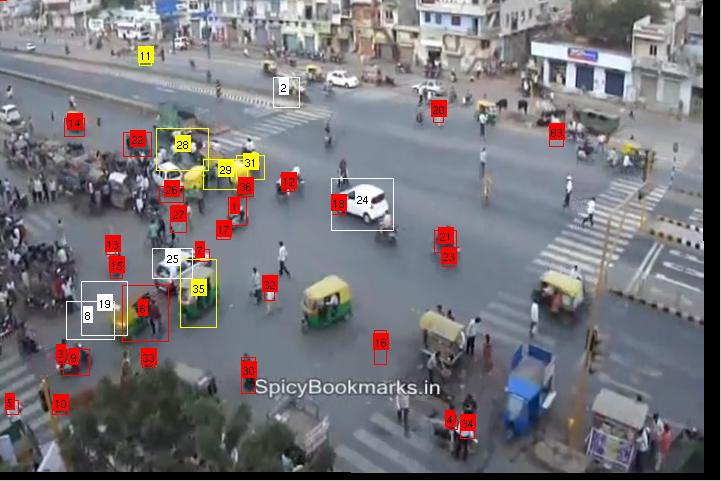
\includegraphics[width=0.5\textwidth]{620.jpg}
\end{figure}

\begin{figure}[h!]
\caption{Frame 640}
\centering
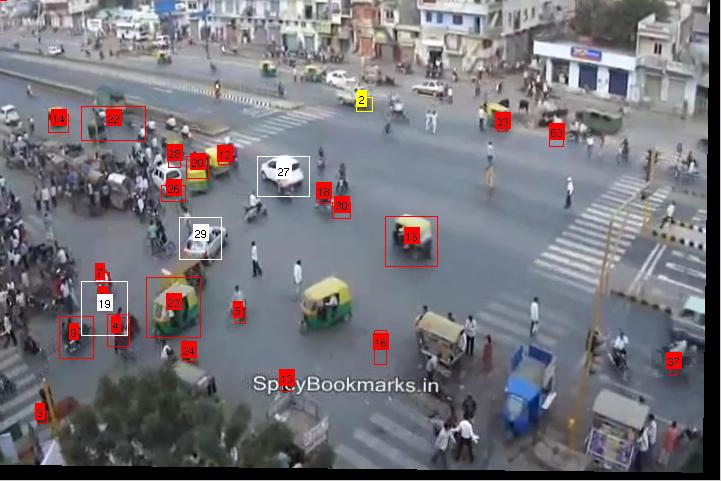
\includegraphics[width=0.5\textwidth]{640.jpg}
\end{figure}

\begin{figure}[h!]
\caption{Frame 720}
\centering
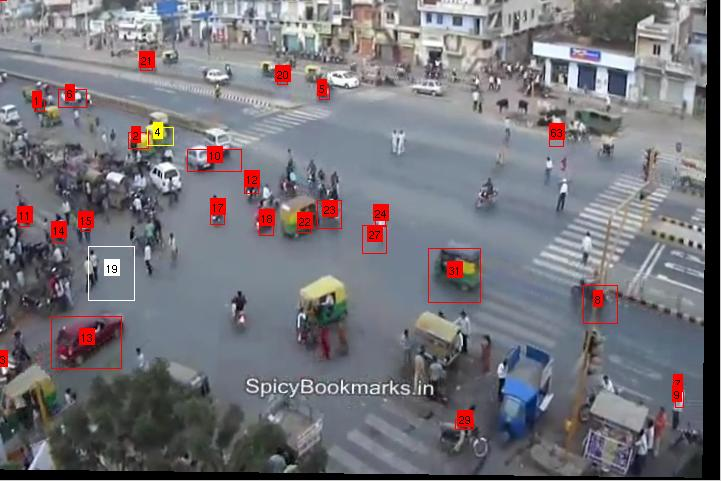
\includegraphics[width=0.5\textwidth]{720.jpg}
\end{figure}

\begin{figure}[h!]
\caption{Frame 740}
\centering
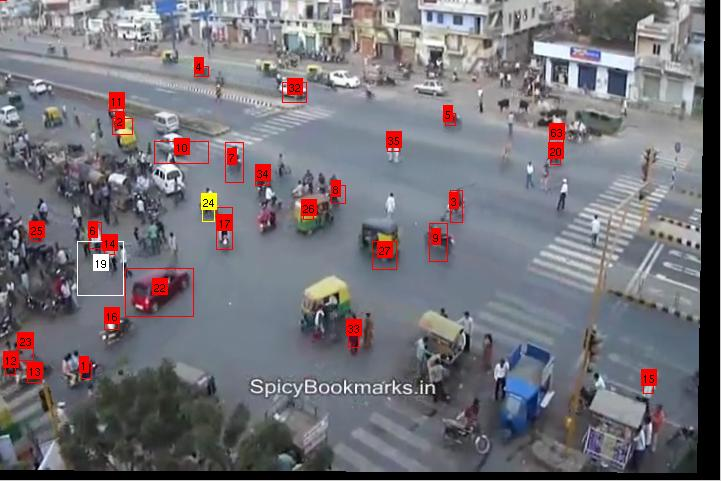
\includegraphics[width=0.5\textwidth]{740.jpg}
\end{figure}

\begin{figure}[h!]
\caption{Frame 840}
\centering
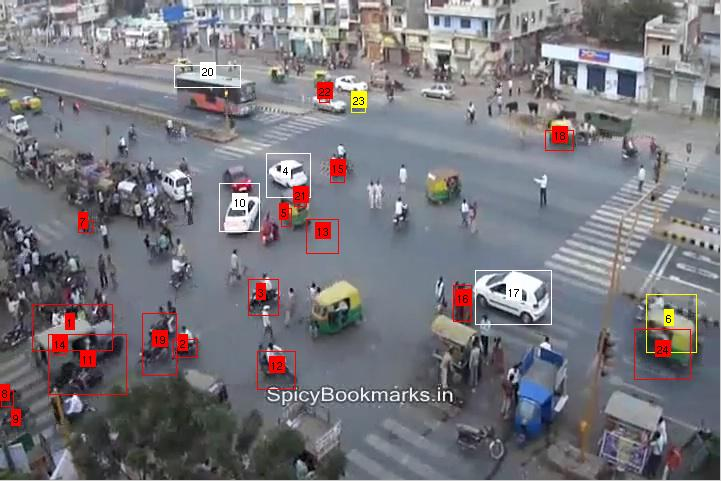
\includegraphics[width=0.5\textwidth]{840.jpg}
\end{figure}

\begin{figure}[h!]
\caption{Frame 860}
\centering
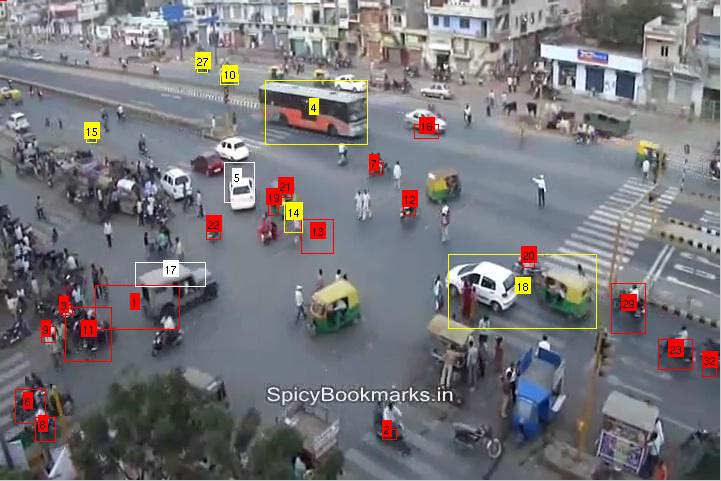
\includegraphics[width=0.5\textwidth]{860.jpg}
\end{figure}

\newpage

\begin{figure}[h!]
\caption{Frame 960}
\centering
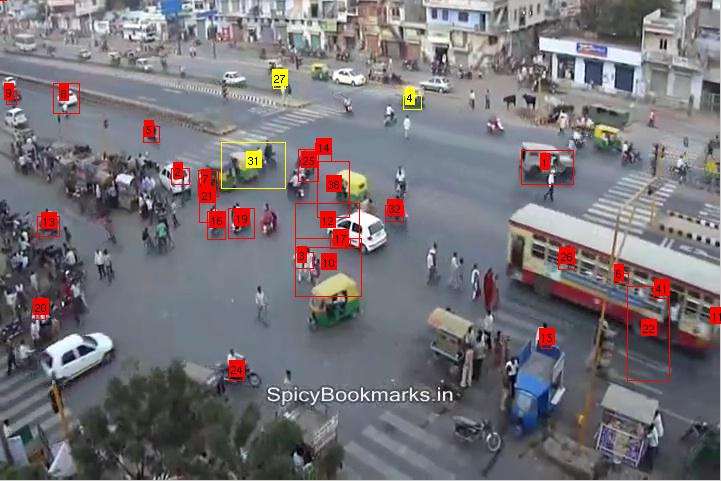
\includegraphics[width=0.5\textwidth]{960.jpg}
\end{figure}

\begin{figure}[h!]
\caption{Frame 980}
\centering
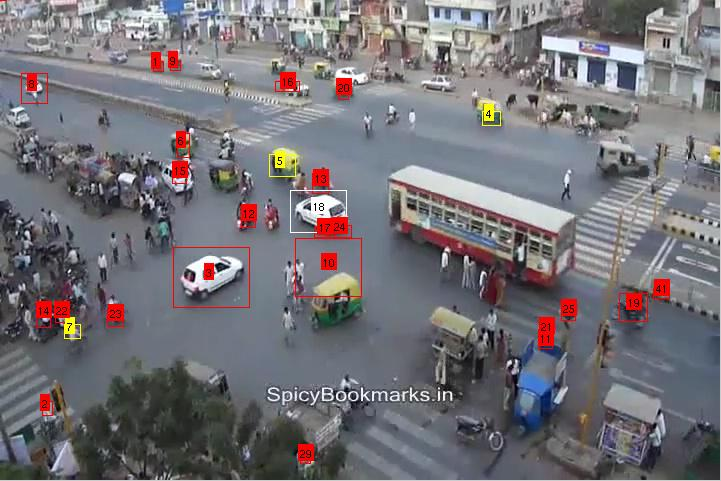
\includegraphics[width=0.5\textwidth]{980.jpg}
\end{figure}




\end{document}
